\documentclass[../norme-di-progetto.tex]{subfiles}
\begin{document}
\subsection{Descrizione}
\label{sub:descrizione}
Sono i processi essenziali durante il ciclo di vita del software. ISO 12207-1995 ne definisce cinque:
\begin{itemize}
	\item Acquisizione
	\item Fornitura
	\item Sviluppo
	\item Gestione operativa
	\item Manutenzione
\end{itemize}
\subsection{Fornitura}
\label{sub:fornitura}
\subsubsection{Finalità}
\label{subs:finalità}
Grupp0ne istanza il processo di fornitura per potersi aggiudicare il capitolato attraverso un accordo con il committente e la successiva stipulazione di un contratto.
\subsubsection{Descrizione}
\label{subs:descrizione}
Il processo di fornitura contiene le attività e i compiti del fornitore. Esso gestisce il rapporto tra il fornitore e il cliente ed inoltre amministra le procedure e le risorse necessarie per lo sviluppo del piano di progetto. È composto da diverse attività:
\begin{itemize}
\item Inizializzazione
\item Preparazione della risposta
\item Contratto
\item Pianificazione
\item Esecuzione e controllo
\item Revisione e valutazione
\item Consegna e completamento
\end{itemize}
\subsubsection{Studio di Fattibilità}
\label{subs:studio di fattibilità}
Grupp0ne si impegna a consegnare un sintetico documento contenente una breve descrizione, i pregi e le criticità riscontrati in ciascuno dei capitolati. Lo studio di fattibilità è redatto dall'\glossario{amministratore}
con l'aiuto degli \glossario{analisti} e ha l'obiettivo di esporre quali capitolati sono stati presi in considerazione con le relative motivazioni. Il documento è così articolato:
\begin{itemize}
\item \textbf{Descrizione}: si fornisce una breve descrizione del problema esposto dal proponente.
\item \textbf{Finalità del progetto}: si descrive che cosa bisogna realizzare.
\item \textbf{Tecnologie interessate}: si mostrano le tecnologie da considerare in fase di sviluppo.
\item \textbf{Aspetti positivi}: si espongono i pregi del capitolato.
\item \textbf{Criticità e fattori di rischio}: si illustrano i difetti osservati studiando il capitolato.
\end{itemize}
\subsubsection{Incontri con il proponente}
\label{subs:incontri con il proponente}
Gruppo0ne intende mantenere uno stretto rapporto di collaborazione con i proponenti del capitolato Stalker. Tale rapporto si mantiene attraverso incontri che si svolgono fisicamente presso le aule del Dipartimento di Matematica ``Tullio Levi Civita'' e virtualmente in hangouts.
Gli obiettivi degli incontri sono:
\begin{itemize}
\item \textbf{Comprensione e perfezionamento dei requisiti}: si vuole discutere col proponente dei problemi e dei dubbi riscontrati durante l`'analisi del capitolato in modo da comprendere incrementalmente i requisiti.
\item \textbf{Ricerca e valutazione del software}: si chiede al proponente se le componenti e i software proposti soddisfino le funzionalità richieste.
\item \textbf{Convalida dei documenti e del prodotto}: ci si rivolge al proponente per avere conferme sul lavoro svolto siano essi documenti, \glossario{prototipi} appena abbozzati o prodotti software ad uno stato avanzato.
\end{itemize}
Gli esiti degli argomenti discussi durante gli incontri saranno poi riportati in verbali.
\subsection{Sviluppo}
\label{sub:sviluppo}
\subsubsection{Finalità}
\label{subs:finalità}
Grupp0ne istanza il processo di sviluppo per realizzare il prodotto richiesto dal proponente.
\subsubsection{Descrizione}
\label{subs:descrizione}
Il processo di sviluppo contiene le attività e i compiti dello sviluppatore. Esso fissa quali sono gli obiettivi dello sviluppo dalla creazione alla consegna del prodotto finale. Raggruppa le seguenti attività:
\begin{itemize}
	\item Analisi dei requisiti
	\item Progettazione
	\item Codifica
	\item Testing
	\item Installazione
\end{itemize}
\subsubsection{Attività}
\label{subs:attività}
\paragraph{Analisi dei requisiti}\mbox{}\\
\label{par:analisi dei requisiti}
\\L'analisi dei requisiti è l'attività che studia e comprende il dominio applicativo del problema e che ha come scopo quello di offrire i requisiti che dovranno essere soddisfatti dal software. Si articola nei seguenti compiti:
\begin{itemize}
	\item Studiare e definire il problema da risolvere
	\item Classificare i requisiti
	\item Realizzare i diagrammi UML dei casi d'uso
	\item Fornire ai progettisti dei requisiti atomici da poter analizzare per iniziare l'attività di progettazione
\end{itemize} 
Il documento di riferimento, \textit{Analisi dei requisiti v1.0.0}, è redatto dagli analisti.
\subparagraph{Classificazione dei requisiti}\mbox{}\\
\label{subp:classificazione dei requisiti}
\subparagraph{Casi d'uso}\mbox{}\\
\label{subp:casi d'uso}
\\ I diagrammi dei casi d'uso descrivono le funzioni e i servizi offerti dal prodotto agli attori che interagiscono con il sistema. Ogni caso d'uso ha :
\begin{itemize}
	\item Una rappresentazione testuale
	\item Una rappresentazione grafica
\end{itemize}
Nel presente paragrafo si descrive la rappresentazione testuale mentre nel successivo verrà descritta la rappresentazione grafica. Un generico caso d'uso è caratterizzato da:
\begin{itemize}
\item \textbf{Titolo}: breve titolo del caso d'uso.
\item \textbf{Codice}: codice identificativo del caso d'uso. Ogni caso d'uso può essere suddiviso in altri sottocasi. La denominazione convenzionale è la seguente:
\begin{itemize}
	\item \textbf{Caso d'uso}: UC[codice numerico].
    \item \textbf{Sottocaso d'uso}: UC[codice numerico del padre].[codice numerico del sottocaso].
\end{itemize}
Ad esempio il primo caso d'uso avrà codice identificativo UC1 mentre i relativi sottocasi saranno UC1.1 UC1.2 UC1.3..
\item \textbf{Attore primario}: attore principale coinvolto nel caso d'uso.
\item \textbf{Attori secondari}(opzionale): attori secondari coinvolti nel caso d'uso.
\item \textbf{Precondizioni}: condizione in cui si trovano gli attori prima del verificarsi del caso d'uso.
\item \textbf{Postcondizioni}: condizione in cui si trovano gli attori dopo il verificarsi del caso d'uso.
\item \textbf{Scenario principale}: sequenza di azioni svolte dall'attore per portare a compimento il caso d'uso.
\item \textbf{Estensioni}(opzionale): sequenza di possibilità dell'attore al verificarsi di eventi anomali o di situazioni di errore.
\end{itemize}
\subparagraph{Diagrammi dei casi d'uso}
\label{subp:diagrammi dei casi d'uso} 
\paragraph{Progettazione}\mbox{}\\
\label{par:progettazione}
\subsubsection{Strumenti}
\label{subs:strumenti}
\paragraph{PlantUml}\mbox{}\\
\label{par:plantuml}
\\ Per la costruzione dei diagrammi dei casi d'uso il team ha deciso di utilizzare PlantUml. È un software open source che permette la costruzione di diagrammi UML a partire dalla scrittura di codice. PlantUml fa uso di GraphViz per la traduzione del plain text in elementi grafici. Grupp0ne ha valutato positivamente tale strumento in quanto:
\begin{itemize}
	\item Permette di scrivere i diagrammi dei casi d'uso sotto forma di codice, mentre il ruolo di costruzione dei diagrammi è demandato al software sottostante.
	\item Permette di scrivere agevolmente non solo i diagrammi dei casi d'uso, ma anche diagrammi delle classi, di sequenza e di package.
\end{itemize}
\begin{figure}[H]
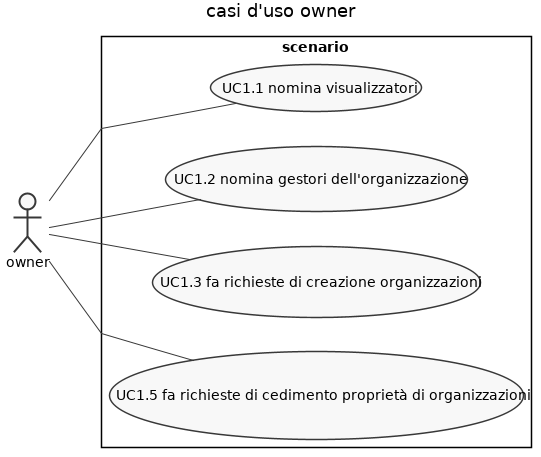
\includegraphics[width=8cm]{components/owner_use_cases.png}
\centering
\caption{diagramma dei casi d'uso realizzato con PlantUml}
\end{figure}
\end{document}